\section{Ergebnisse}
\subsection{Messung des Dunkelstroms in Abh"angigkeit von der Temperatur}
Zunächst wurden bei einer Belichtungszeit von 30 Sekunden dark frames bei verschiedenen Temperaturen des Chips aufgenommen, um die ideale Betriebstemperatur des CCD zu ermitteln. Eine beispielhafte Aufnahme bei -3 $^\circ$ \, C ist in Abb. \ref{fig:dark} dargestellt. 

\begin{figure}[h!]
\centering
        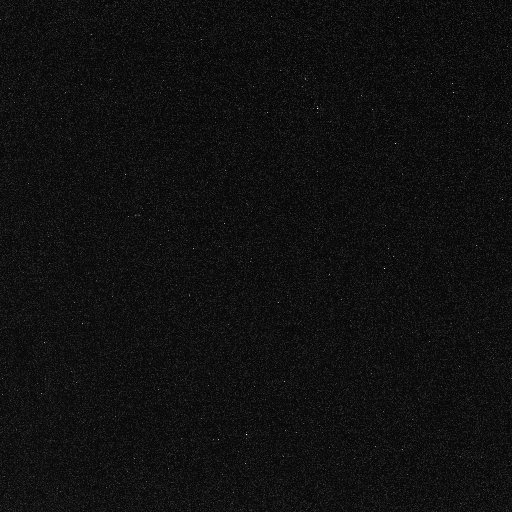
\includegraphics[width=.5\textwidth]{dark.png}
\caption{ Aufnahme eines dark frames bei -3  $^\circ$ C}
\label{fig:dark}
\end{figure}

Hierbei ergaben sich die in Tabelle \ref{tbl:adu_temp} dargestellten Werte, welche in Abb. \ref{fig:adu_temp} graphisch dargestellt sind. 
\begin{figure}[h!]
\centering
        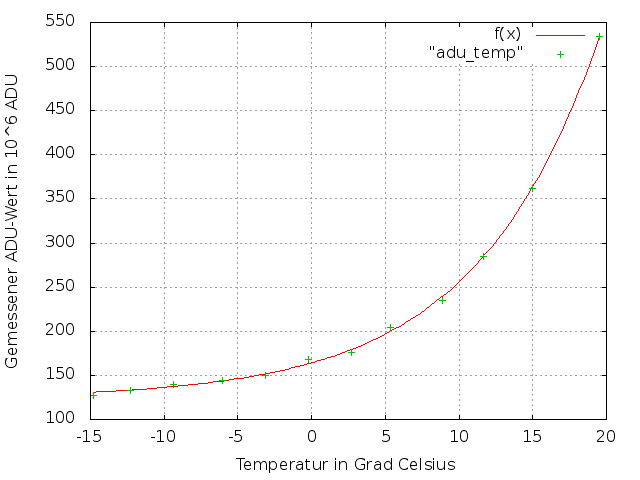
\includegraphics[width=.9\textwidth]{plot_adu_temp2.png}
\caption{ Auftragung von Dunkelstrom über der CCD-Temperatur }
\label{fig:adu_temp}
\end{figure}
Hier wurde der Verlauf mit einer Exponentialfunktion $f(T) = a \cdot \exp(T \cdot c) + b$ gefittet, welche theoretisch zu erwarten ist, da die Energie der Elektronen im Halbleiter prinzipiell Boltzmann-verteilt ist. \\
Es ergibt sich also eine ideale Temperatur von etwa -15 $^\circ$ C im betrachteten Intervall von -15 bis + 20 $^\circ$ C. Eine tiefere Temperatur ist aufgrund der begrenzten Kühlleistung des CCD-Chips nicht erreichbar. Für die Fitparameter ergibt sich: 
$a = 40.0\  \mathrm{adu}, c = 0.119 \frac{1}{\mathrm{K}}, b = 124.2 \ \mathrm{adu}$.\
Augenscheinlich approximiert der Fit die Messdaten sehr gut, die variance of residuals ergibt sich nach gnuplot zu 12.06. 
\subsection{Bestimmung des Bias}
Die Aufnahme eines bias frames bei einer Belichtungszeit von 0.12 s ist in Abb. \ref{fig:bias} zu sehen, wobei die Helligkeit zur besseren Darstellung erh"oht wurde. 
\begin{figure}[h!]
\centering
        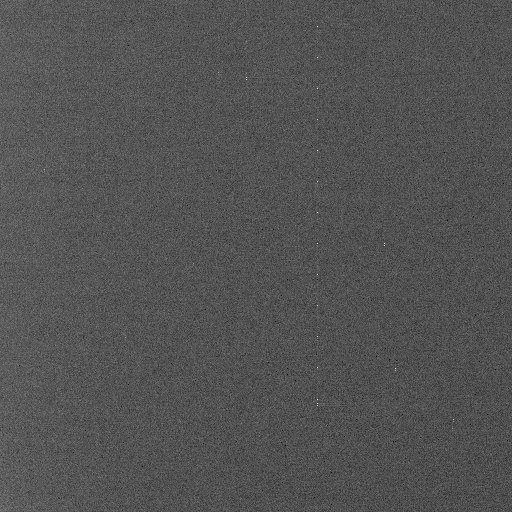
\includegraphics[width=.5\textwidth]{beiers_01.png}
\caption{ Aufnahme eines bias frame }
\label{fig:bias}
\end{figure}
Neben dem Rauschen im Hintergrund erkennt man mehrere senkrechte gepunktete Linien. Diese sind auf ein hot pixel in der entsprechenden Spalte zurückzuführen. Aufgrund des \enquote{schubweisen} Auslesens der Zeilen, welches laut dem Betreuer durch Speicherüberläufe in der Ausleseelektronik verursacht wird, kommt es in regelmäßigen zeitlichen Abständen zu einer Verzögerung beim Auslesen und somit zu hellen Punkten mit räumlich gleichem Abstand. Des weiteren ist ein leichter Helligkeitsgradient von links nach rechts sichtbar. Der Grund hierfür ist wahrscheinlich ein Temperaturgradient im CCD-Chip und ein somit räumlich unterschiedlicher Dunkelstrom. Eine weitere Erkl"arung w"are ein Elektronenverlust beim Auslesen der Zeile, sodass die zuerst ausgelesenen Pixel heller als die nachfolgenden erscheinen.\\
Es wurden insgesamt 11 bias frames aufgenommen, deren mittlerer ADU-Wert sich zu 115.6 $ \pm 1.07$ ergibt, wobei der hier angegebene Fehler die Standardabweichung der ADU-Werte ist. \\\
\subsection{Bestimmung des Gain-Faktors}
Hierzu wurden zu verschiedenen Belichtungszeiten je zwei flat field-Aufnahmen eines homogen ausgeleuchteten Blatts Papier angefertigt.
Damit auch bei maximaler Belichtungszeit kein überbelichtetes Bild aufgenommen wurde, musste insgesamt ein Filter der Stärke 2048, der also nur $\frac{1}{2048}$ des Lichts transmittiert, verwendet werden. 
Zur Bestimmung des Gain-Faktors werden zu jeder Belichtungsdauer je zwei flat fields aufgenommen und ausgewertet. Dabei ergeben sich mit der Formel \eqref{form:gain} die in Tabelle \ref{tbl:gain} dargestellten Werte. \\
F"ur den Fehler wurde der Fehler von $N_{ADU}(A)$, $N_{ADU}(C)$, $N_{ADU}(\overline{B_1})$, $N_{ADU}(\overline{B_2})$ sowie eine auf \eqref{form:gain} aufbauende Fehlerfortpflanzung verwendet:
\footnotesize
\begin{align}
\delta g = \nonumber\\&= \sqrt{(\frac{1}{\sigma_{ADU}^2(A-C) - \sigma_{ADU}^2(B_1-B_2)})^2 \cdot (\delta N_{ADU}(A)^2 + \delta N_{ADU}(C)^2+ \delta N_{ADU}(\overline{B_1})^2 + \delta N_{ADU}(\overline{B_2})^2)}. 
\end{align}
\normalsize
Hierbei wurden nur f"ur die im Z"ahler vorkommenden Werte Fehler verwendet. F"ur die Standardabweichungen im Nenner ist es schwierig, Fehler zu bestimmen, sodass diese nicht in der Fehlerfortpflanzung verwendet werden. 

Als gemittelter Wert ergibt sich 
\begin{equation}
\bar{g} = 1.94 \pm 0.04 \ \frac{\mathrm{ADU}}{\mathrm{e}}. 
\end{equation}
Die Werte für den Gain-Faktor sind zwar alle im gleichen Bereich, es ist aber eine leichte Tendenz zu kleineren Gain-Faktoren bei größeren Belichtungszeiten erkennbar. Der Grund hierfür dürfte in Fehlern, die sich in der statistischen Betrachtung zur Herleitung der Formel für den Gain-Faktor ergeben, liegen. 
\subsection{Untersuchung der Linearit"at des CCDs}
In Tabelle \ref{tbl:adu_int} sind die gemessenen ADU-Werte aufgetragen über dem transmittierten Licht als Anteil der Lichtintensität, wobei die Helligkeit "uber einer rechteckigen Fl"ache, die die gesamte Diode einschlie"st, aufintegriert wurde. Da, laut dem Betreuer, die Werte f"ur die aufintegrierte Intensit"at Poisson-verteilt ist, ergibt sich der Fehler als Quadratwurzel der gemessenen und aufintegrierten ADU-Werte. \\
Plottet man die ermittelten Werte, so ergibt sich der in Abb. \ref{plot:adu_int} dargestellte Verlauf. Werden die Datenpunkte mit der Funktion 
\begin{equation}
f(x) = a \cdot x + b
\end{equation}
gefittet, so ergeben sich die Werte $a = (119 \pm 5.0) \cdot 10^6 \ ADU$ und $b = (2.8 \pm 1.4) \cdot 10^6 \ ADU$.
\begin{figure}[h!]
\centering
        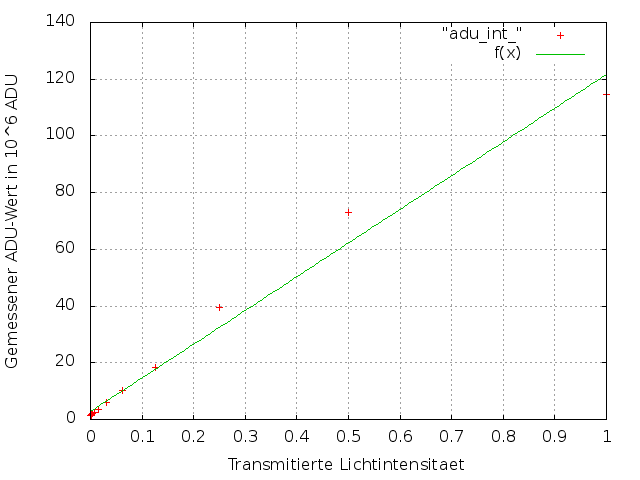
\includegraphics[width=.9\textwidth]{adu_int_.png}
\caption{ Auftragung des gemessenen ADU-Wertes über der einfallenden Lichtintensität }
\label{plot:adu_int}
\end{figure}
Der Fit approximiert die Punkte nahe der Null sehr gut, die Punkte mit h"oherer Intensit"at jedoch eher schlecht. Grund hierf"ur ist insbesondere der Wert bei Intensit"at 1, d.h. ohne Filter. M"oglicherweise fand hier trotz entsprechender Blendeneinstellung von 5.6f eine "Uberbelichtung statt. Die variance of residuals ergibt sich zu 18.9. \\
\subsection{Blooming und Smear}
\begin{figure}[h!]
\centering
        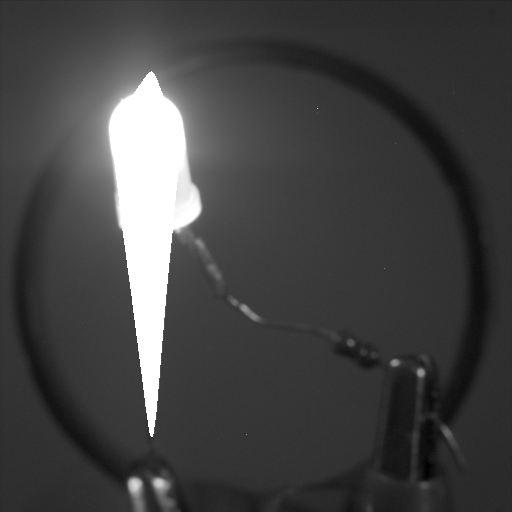
\includegraphics[width=.4\textwidth]{blooming2.png}
\caption{ Aufnahme der Diode bei extremer Überbelichtung }
\label{fig:blooming}
\end{figure}
In Abbildung \ref{fig:blooming} (logarithmische Darstellung) ist eine Aufnahme der Diode bei starker Überbelichtung dargestellt, was durch eine Belichtungszeit von 5 Sekunden und einer Blende von 8f erreicht wurde. Man erkennt, dass nicht nur die tatsächlich überbelichteten Pixel hell sind, sondern auch die spaltenweise benachbarten Pixel. Der Grund hierfür ist, dass die Potentialtöpfe der einzelnen Pixel schlicht \enquote{überlaufen}, sodass Elektronen in benachbarte Pixel wandern. Dies geschieht vor allem innerhalb der Spalten und nur wenig in den Zeilen, da diese gegeneinander isoliert sind. Im Gegensatz dazu werden die Elektronen in den Spalten verschoben, sodass diese nicht isoliert sein dürfen. \\ \\
Zur Veranschaulichung des Smear-Effektes wurden Aufnahmen bei deaktiviertem Shutter, einer Belichtungszeit von 0.5 Sekunden und ebenfalls einer Blende von 8f gemacht, wobei der Strahlengang zunächst durch ein Blatt Papier unterbrochen war, dass dann entfernt wurde. Die Ausleseelektronik befindet sich hier am oberen Bildrand. 
Bei der ersten Aufnahme zeigte sich das in \ref{fig:smear1} dargestellte Bild (hier in logarithmischer Darstellung). 

\begin{figure}[h!]
\centering
        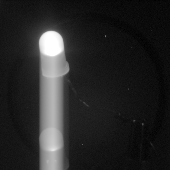
\includegraphics[width=.4\textwidth]{smear_unten_sebi2.png}
\caption{ Erste Aufnahme nach Belichtungsbeginn }
\label{fig:smear1}
\end{figure}
Der Effekt erklärt sich folgendermaßen:\\
An eine Belichtung des CCD-Chips schlie"st sich ein Auslesevorgang an, w"ahrend dem der Chip weiter beleuchtet wird, da der Shutter ge"offnet ist. Zu Beginn des Auslesens sind die ersten ausgelesenen Pixel unbelichtet. Wird das erste stark belichtete Pixel ausgelesen, so ergibt sich ein heller Punkt. Die diesem Pixel nachfolgenden Pixel wurden, da der Shutter ge"offnet war, während des Auslesens weiter belichtet, sodass sie heller als der Hintergrund erscheinen. Diese Pixel liegen vom stark belichteten Pixel entgegen der Ausleserichtung. \\
Bei der zweiten Aufnahme ist dann ein durchgehender \enquote{smear} erkennbar, was daran liegt, dass die Pixel vor dem stark belichteten Pixel noch während des vorhergehenden Ausleseprozesses belichtet werden, sodass noch vor der eigentlichen Belichtung sich bereits Elektronen in den Potentialt"opfen befinden. Somit erscheint ein durchgehend heller Strich in der Spalte. Dies ist in Abb. \ref{fig:smear2} (ebenfalls in logarithmischer Darstellung) dargestellt. 

\begin{figure}[h!]
\centering
        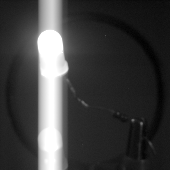
\includegraphics[width=.4\textwidth]{smear2.png}
\caption{ Zweite Aufnahme }
\label{fig:smear2}
\end{figure}

Wird nun das Blatt Papier w"ahrend (hier eher zum Ende) der Belichtung in den Strahlengang eingeführt, so ergibt sich die in Abb. \ref{fig:smear3} (ebenfalls logarithmisch) dargestellte Aufnahme. 

\begin{figure}[h!]
\centering
        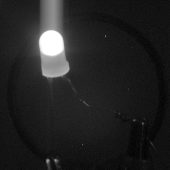
\includegraphics[width=.4\textwidth]{smear_oben2.png}
\caption{ Aufnahme nach Einführen des Blattes }
\label{fig:smear3}
\end{figure}
Der Grund f"ur diese Erscheinung ist zun"achst, dass die oberen Pixel wiederum während des vorherigen Auslesens belichtet werden und somit hell erscheinen. Auch das prim"are Bild der Diode ist sichtbar, da der Strahlengang erst am Ende der Belichtungszeit unterbrochen wurde. Nach dem Einführen des Blattes in den Strahlengang werden keine weiteren Pixel belichtet, sodass der smear-Effekt unterhalb der Diode nicht auftritt, das Blatt ersetzt quasi den Shutter der Kamera. 
